\documentclass{report}

\usepackage[utf8]{inputenc}
\usepackage[francais]{babel}
\usepackage{graphicx}

\renewcommand{\thesection}{\arabic{section}}
\begin{document}
\title{%
    \begin{minipage}\linewidth
        \centering
        Compte-Rendu TD-03 
        \vskip 3pt
        \large Java-Création d'un simulateur de pokémon
        \author{BOURDELAS Pablo, ROUIBAA Doha, et RYCKAERT Guillaume}
    \end{minipage}
\begin{figure}[ht!]
    \centering
    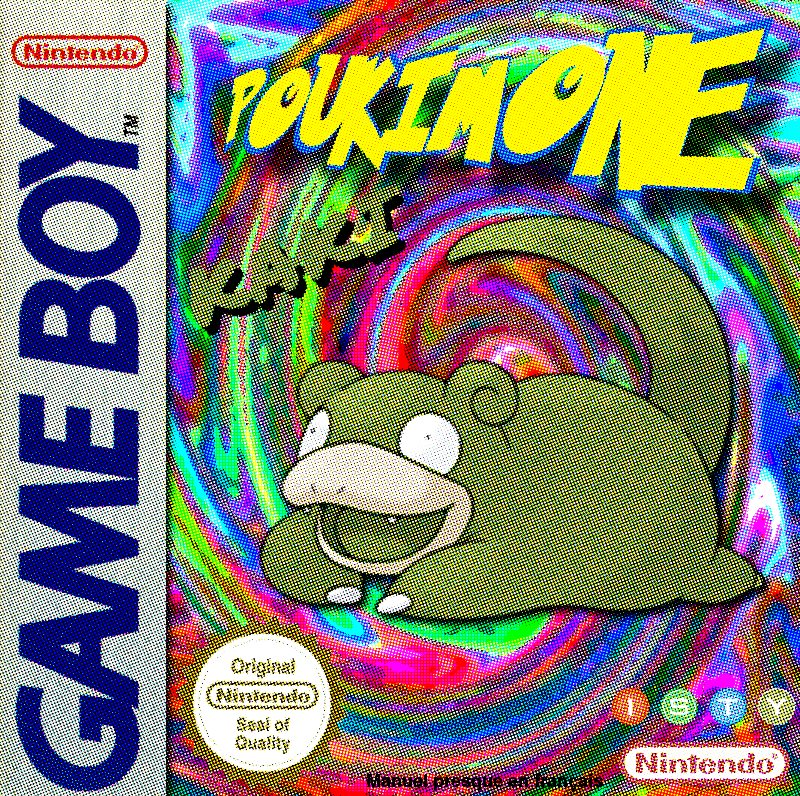
\includegraphics[width=75mm]{cover.jpg}
\end{figure}
    }   

\maketitle

\chapter*{Avant-Propos}
Toute ressemblance avec des jeux, systèmes et créatures imaginaires ayant existé est PUREMENT fortuit, et ne peux être considéré comme plagiat de la part des auteurs.\\
Poukimone est une marque déposée par Sean Juy Gayous et CRLYPS Ltd, Hong Kong, Tout droits réservés, des poursuites par cours de conception pourront être entreprises.
 
\newpage
\section*{Question 1}

Nos Poukimone reposent sur 2 classes.
\subsection*{Stats}
Cette classe contient les stats du Poukimone.Chaque Poukimone est est associé a deux instances de cette classe, l'une contenant les Statistiques de base du poukimone (au niveau 1), l'autre contenant celles actuelles (calculées a partir de celles de base).
\subsection*{Poukimone}
Cette classe sert a stocker les caractétistiques permanantes du Poukimone, qui ne changeront jamais au cours du temps.\\ 
Elle contient notemment:
\begin{itemize}
    \item{Le nom du Poukimone}\\
    \item{La courbe d'experience du Poukimone}\\
    \item{Le type du Poukimone}\\
    \item{Le nombre de points d'experience requis pour passer au niveau suivant}\\
    \item{Ses statistiques, stockées via la classe ci-dessus}\\
    \item{Ses Capacités}
\end{itemize}


\begin{figure}[ht!]
    \centering
    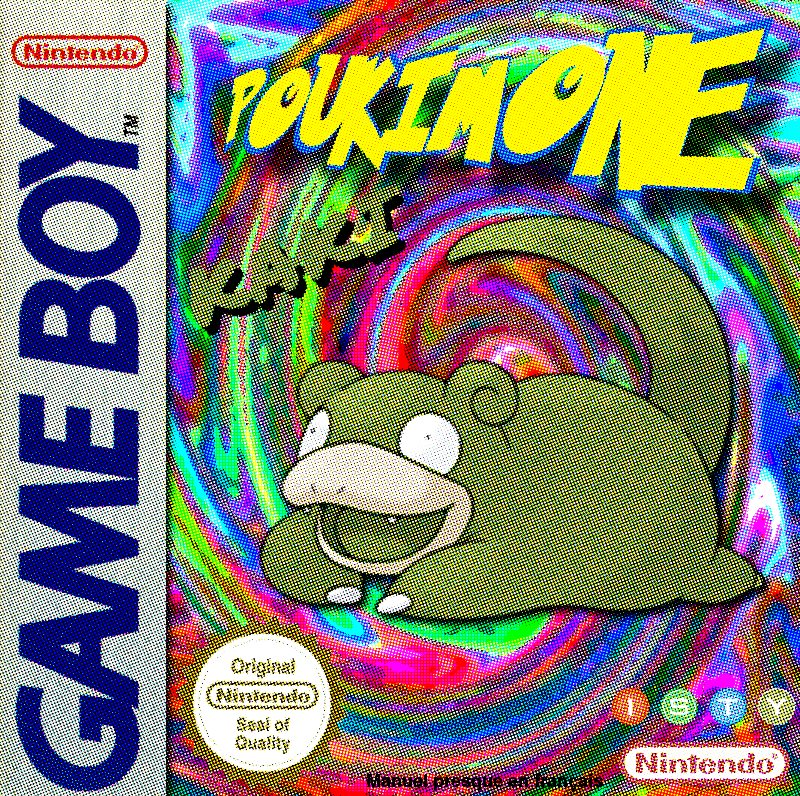
\includegraphics[width=60mm]{cover.jpg}
    \caption{"Schéma de classe du projet"}
\end{figure}
\newpage
\section*{Question 2}
Notre Pokémon possède de nombreux attributs, la plupart sont stockés dans deux instanses de la classe Stats. Une de ses instances contient les stats de base du Poukimone. L'autre contient ses attributs calculés au niveau actuel.
\\Cette classe stats contient les attributs suivants:
\begin{itemize}
    \item{Pv max, attaque, defense, vitesse}
    \item{Niveau}
    \item{Points d'expérience accumulés, Ou, pour l'instance associée au stats de base, la base de points d'experience rapportée lorsque ce Poukimone est vaincu.}
    \item{Pv actuels}
\end{itemize}
D'autres attributs sont contenus en dehors de cette classe, comme le type de courbe d'xp, l'experience requise pour passer au niveau suivant, le nom du Poukimone, son type, ainsi que ses 4 capacités.
\\ Toutes ces statistiques sont obtenues a partir d'un fichier json contenant les stats de base de tous les Pokémons de la G1
\section*{Question 3}
\subsection*{Méthodes liées aux caractéristiques}

\begin{itemize}
    \item{get\_base:}
        Cette méthode sert a récupérer toutes les statistiques de base d'un Poukimone donné. Etant relativement lente, nous essayons d'y faire le moins appel possible.\\
    \item{calc\_exp:}
        A partir du niveau du Poukimone, ainsi que de la nature de sa courbe d'experience, cette méthode met a jour le nombre de points d'experience requis pour passer au niveau suivant.\\
    \item{level\_up:}
        Fait passer le Poukimone au niveau supérieur, en mettant a jour ses stats ainsi que la valeur d'xp requise pour passer au niveau suivant.\\
    \item{set\_level:}
        Met un Poukimone au niveau donné par appel successifs de level\_up.
\end{itemize}
\subsection*{Méthodes liées au combat}
\begin{itemize}
    \item{take\_damage:}
        Cette méthode gère les dégats pris par le Poukimone. Elle prend en entrée les Poukimone ennmi, et la puissance de l'attaque, et déduit les dégats de la vie du Poukimone.\\
    \item{use\_ability:}
        Cette méthode lui sert a attaquer,via la classe Ability.\\
    \item{kill:}
        Tue instentanément le Poukimone.\\
    \item{is\_dead:}
        retourne vrai si le Poukimone n'as plus de vie.
\end{itemize}
\subsection*{Autres méthodes}
\begin{itemize}
    \item{Constructeur:}
        Crée un Poukimoke de type et de niveau donné.\\
    \item{add\_ability:}
        Ajoute une capacitée donnée au Poukimone.\\
    \item{list\_abilites:}
        Liste les capacitées du Poukimone.
\end{itemize}
\section*{Question 4}
\begin{figure}[ht!]
    \centering
    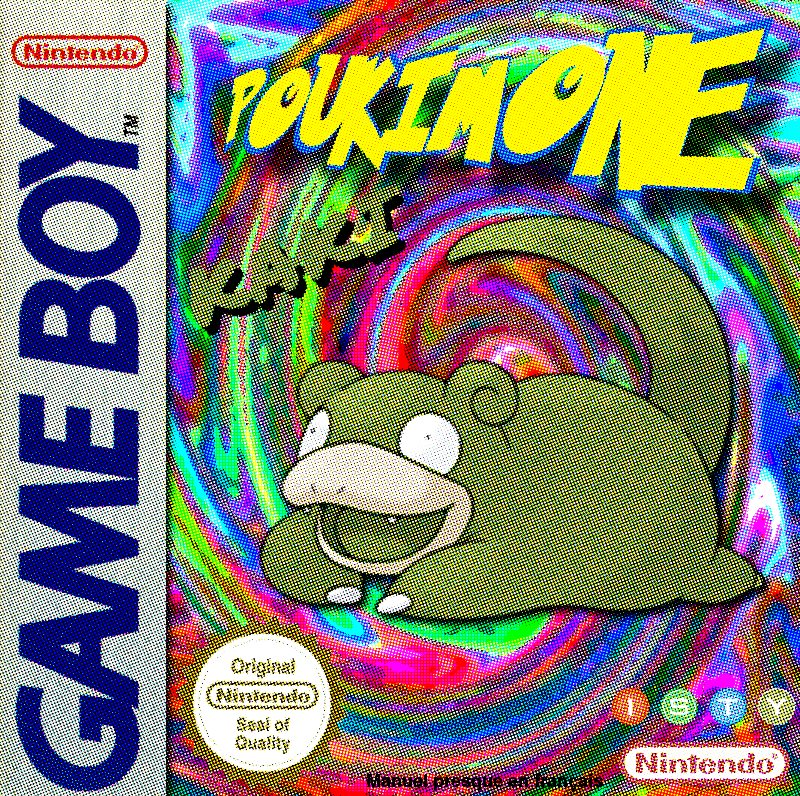
\includegraphics[width=60mm]{cover.jpg}
    \caption{"Schéma de classe du projet, avec les capacités"}
\end{figure}


\section*{Question 6}
Notre programme contient une classe Fight, dont le constructeur appelle le premier tour, en fonction de la vitesse des poukimone. La classe apelle enuite le tour du joueur advers, et ainsi de suite... jusqu'a la mort d'un des deux Poukimone.

\chapter*{Le texte que j'ai déja écrit qui peut servir plus tard... (ça sert de lire les questions avant d'y répondre... :/}
\subsection*{Ability}
Cette classe sert a gérer les capacités des Poukimones.Elle gère la puissance, la précision,le type, et le nombre de pp de la capcité.
\subsection*{Bag}
Cette classe gère l'inventaire du joueur.Elle gère les potions et les huiles.
\subsection*{Type}
Cette classe gère les types de Poukimone et des Capacités.
\subsection*{Trainer}
Cette classe contient le nom du dresseur, son inventaire, ainsi que son équipe de poukimone.
\subsection*{Fight}
Cette classe sert a gérer le combat.\\



\end{document}
